%---------------------------------------------------------------------------%
%---------------------------------------------------------------------------%
%                          MPT THEME - EXAMPLE                              %
%---------------------------------------------------------------------------%
%---------------------------------------------------------------------------%

%---------------------------------------------------------------------------%
% HEADER                                                                    %
%---------------------------------------------------------------------------%

%----- DOCUMENT TYPE--------------------------------------------------------%
%---------------------------------------------------------------------------%

\pdfminorversion = 5
\documentclass[10pt]{beamer}
\usetheme[francais %[For documents written in french]
%,notocfoot %[To remove the presentation title in the footer of the frames]
%,arial %[To use arial as the default text font instead of Linux Biolinum]
,alertred %[For the alterted text to be framed in red instead of blue]
%,euler %[To use euler as the default math font instead of XITS]
%,sober %[To remove the grey areas behind the frame titles and the footer]
]{MPTM} %[Comment and uncomment options as desired]


%----- PACKAGES-------------------------------------------------------------%
%---------------------------------------------------------------------------%
% [Put all desired packages here]

%Notes
\usepackage{pdfpages}
%\setbeameroption{show notes} %[to show note on the pdf]
%\setbeameroption{show notes on second screen=right}%Pour placer les notes à droite, en extension d'une slide mais commande qui ne marche pas


%TIKZ
\usepackage{pgfplots}

\pgfplotsset{compat=1.14}

\usetikzlibrary{calc, 3d, positioning, intersections, backgrounds, shapes, math, shapes.geometric, topaths, decorations.markings, pgfplots.colormaps}
\usepgfplotslibrary{colormaps, fillbetween}
\pgfplotsset{probastyle/.style={smooth, width = \textwidth, axis x line = bottom, axis y line = left,
		every axis x label/.style={ at={(ticklabel* cs:1.05)}, anchor=west,},
		every axis y label/.style={	at={(ticklabel* cs:1.05)}, anchor=south,}}}
\pgfplotsset{ colormap={MPT}{rgb255(0cm)=(0,94,158) rgb255(0.25cm)=(0,111,182) rgb255(1cm)=(240,240,240) rgb255(2cm)=(156,158,159)}}
\pgfplotsset{compat=newest}
\pgfplotsset{school/.style={tick align = outside, major tick length = 2.5pt, axis line style={-stealth}, anchor = center, x label style = {anchor = west, at = {(current axis.right of origin)}}, y label style = {anchor = south, at = {(current axis.above origin)}, rotate = -90}}}
\usepackage{tikz-3dplot}
\tdplotsetmaincoords{60}{-30}
\tdplotsetrotatedcoords{0}{90}{90}
\pgfmathdeclarefunction{gaussShape}{2}{%
  \pgfmathparse{(1/#2)*exp(-((x-#1)^2)/(1^2))}%
  }
  \pgfmathdeclarefunction{gauss}{2}{%
  \pgfmathparse{(1/(#2*sqrt(2*pi)))*exp(-((x-#1)^2)/(2*#2^2))}%
}
\tikzset{
		    base/.style = {draw=MPTgrey, ultra thick, 
			minimum height=30mm, minimum width=30mm,
			inner sep=0pt}, %permet d'afficher une image dans un rectangle
  invisible/.style={opacity=0},
  visible on/.style={alt={#1{}{invisible}}},
  alt/.code args={<#1>#2#3}{%
    \alt<#1>{\pgfkeysalso{#2}}{\pgfkeysalso{#3}} % \pgfkeysalso doesn't change the path
  },
}
\usetikzlibrary{arrows.meta}

%smiley souriant bleu
\newcommand{\smiley}{\tikz[baseline=-0.75ex,black]{
		\draw[MPTblue] circle (2mm);
		\node[MPTblue,fill,circle,inner sep=0.5pt] (left eye) at (135:0.8mm) {};
		\node[MPTblue,fill,circle,inner sep=0.5pt] (right eye) at (45:0.8mm) {};
		\draw[MPTblue] (-145:0.9mm) arc (-120:-60:1.5mm);
	}
}

%smiley pas content rouge
\newcommand{\frownie}{\tikz[baseline=-0.75ex,black]{
		\draw[MPTred] circle (2mm);
		\node[MPTred,fill,circle,inner sep=0.5pt] (left eye) at (135:0.8mm) {};
		\node[MPTred,fill,circle,inner sep=0.5pt] (right eye) at (45:0.8mm) {};
		\draw[MPTred](-145:0.9mm) arc (120:60:1.5mm);
	}
}


%----- MATH
%\usepackage{amsmath, amssymb, amscd, latexsym, bigints, stmaryrd, bm}
\usepackage{stmaryrd, bm}

\let\oldoverrightarrow\overrightarrow
\renewcommand{\overrightarrow}[2][]{{%
		\if$#1$\else\color{#1}\fi% Optional argument given...
		\oldoverrightarrow{\color{black}#2}%
}}

%----- TABLES
\usepackage{booktabs, tabularx, multirow, colortbl}
\arrayrulecolor{main}
\setlength{\aboverulesep}{0pt}
\setlength{\belowrulesep}{0pt}
\setlength{\extrarowheight}{5pt}
\newcolumntype{L}{>{\raggedright\arraybackslash}X}
\newcolumntype{R}{>{\raggedleft\arraybackslash}X}
\newcolumntype{C}{>{\centering\arraybackslash}X}
\newcolumntype{s}{@{\hspace{3pt}} c @{\hspace{6pt}}}

%----- FIGURES
\usepackage{graphicx, psfrag, color, epsfig}   % to include and manipulate graphics
\usepackage[all]{xy}    % to draw diagrams
%\usepackage{ifsym}
\usepackage{multirow}

%----- LISTS
\usepackage{enumerate}
%\usepackage{enumitem}

%----- BIBLIO
\usepackage{bibentry}

%-----BARRER
\usepackage{soul}

%----- SYMBOLS
\usepackage{pifont}
\usepackage{bclogo}

%----Font
\usepackage{verbatim}
\usepackage{fancyvrb}
\makeatletter
\newcommand{\verbatimfont}[1]{\renewcommand{\verbatim@font}{\ttfamily#1}}
\makeatother

%-----color href
\hypersetup{colorlinks,linkcolor=,urlcolor=MPTblue}


%----- ADDITIONAL COMMANDS 
%---------------------------------------------------------------------------
\newcommand{\bfun}{\bm{1}}
%\let\sectionOld\section
%\renewcommand\section[2][\empty]{%boldmath\sectionOld[#1]{#2}\unboldmath%}
% [Put all user-defined commands here]

%----- Symbols
\newcommand{\ex}{{\color{MPTblue}\ding{228}}}
%\newcommand{\ex}{{\color{MPTblue}\small{\blacktriangleright}}}

%----- SPACES
\newcommand{\hsp}{\hspace*{1em}}
\newcommand{\midhsp}{\hspace*{.5em}}

\makeatletter
\define@key{beamerframe}{c}[true]{% centered
	\beamer@frametopskip=0pt plus 1fill\relax%
	\beamer@framebottomskip=0pt plus 1fill\relax%
	\beamer@frametopskipautobreak=0pt plus .4\paperheight\relax%
	\beamer@framebottomskipautobreak=0pt plus .6\paperheight\relax%
	\def\beamer@initfirstlineunskip{}%
}
\makeatother



%----- BIBLIO
\newcommand{\itbib}[1]{{\itshape \bibentry{#1}}}
%\providecommand{\bysame}{S.I. Resnick}%

%----- PATHS
%---------------------------------------------------------------------------%
\graphicspath{{Images/}}	%[Indicate the name of the file where your images are stored]

%---------------------------------------------------------------------------%
% TITLE                                                                     %
%---------------------------------------------------------------------------%

\title{Classification supervisée et non supervisée}
\subtitle{
	{Clustering}}
\author{Marine Demangeot}
%\institute{Mines ParisTech}{Equipe Géostatistique}{}
%\coauthor{Sophie Lèbre}
%\coauthor[2]{Anne Sabourin}
%\coinstitute{Mines ParisTech}{Equipe Géostatistique}{}
%\coinstitute[2]{Telecom Paris}{Equipe S2A}{}
\date{25/09/2022}
\event{M1 MIASHS}
%\subtitle{Subtitle}
\rclogo{}	% Research center(s) logo(s)
\netlogo{}	% Partner(s)  logo(s) separated by comma

%---------------------------------------------------------------------------%
% PRESENTATION                                                              %
%---------------------------------------------------------------------------%
\begin{document}
	
%---------------------------------------------------------------------------%
% TITLE FRAME                                                               %
%---------------------------------------------------------------------------%
\begin{frame}
	\maketitle
\end{frame}

%---------------------------------------------------------------------------%
% TOC SETUP                                                                 %
%---------------------------------------------------------------------------%

%Ce qui est affiché quand on a la commande \section{}

\AtBeginSection[]{
	{
		\usebackgroundtemplate{
			\begin{tikzpicture} [inner sep = 0pt, outer sep = 0pt]
			
			%----- MASK - \pgflinewidth
			\node [anchor = north west, minimum width = \paperwidth - \pgflinewidth, minimum height = \paperheight - \pgflinewidth] (pc) at (current page.north west) {};
			
			%----- BACKGROUND
			\shade[top color = event.bg, bottom color = white] (pc.north west) rectangle ([yshift = -15pt]pc.north east);
			\shade[bottom color = event.bg, top color = white] (pc.south west) rectangle ([yshift = 15pt]pc.south east);
			
			----- SECTION NUMBER %[Uncomment if you want the section number to appear in the background]
			\node[minimum height = .9\paperheight, anchor = center] at (current page.center) {\color{event.bg}{\fontsize{300}{0}\selectfont\Roman{section}}};
			
			%----- TITLE SECTION
			\node[anchor = center, text centered] at (current page.center) {\begin{minipage}[c]{.9\textwidth} \centering \huge\bfseries\scshape\color{MPTblue}\insertsection
			\end{minipage}};
			
			%%----- BACK/PROB/STAT/ALGO %pour rajouter des logos sur la page de section
			%\node[anchor = north west] at ([xshift = 1em, yshift = -2em]current page.north west) {
%				\ifnumequal{\value{section}}{1}{
\includegraphics[width = 2cm]{Back.pdf}}{}
			%};
			\end{tikzpicture}
		}
		\begin{frame}[noframenumbering, plain]
			
		\end{frame}
	}
}


%Ce qui est affiché quand on a la commande \subsection{}
\AtBeginSubsection[]{
	{
		\usebackgroundtemplate{
			\begin{tikzpicture} [inner sep = 0pt, outer sep = 0pt]
				
				%----- MASK - \pgflinewidth
				\node [anchor = north west, minimum width = \paperwidth - \pgflinewidth, minimum height = \paperheight - \pgflinewidth] (pc) at (current page.north west) {};
				
				%----- BACKGROUND
				\shade[top color = event.bg, bottom color = white] (pc.north west) rectangle ([yshift = -15pt]pc.north east);
				\shade[bottom color = event.bg, top color = white] (pc.south west) rectangle ([yshift = 15pt]pc.south east);
				
				----- SECTION NUMBER %[Uncomment if you want the section number to appear in the background]
				\node[minimum height = .9\paperheight, anchor = center] at (current page.center) {\color{event.bg}{\fontsize{300}{0}\selectfont \scshape{\alph{subsection}}}};
			
			%----- TITLE SUBSECTION
			\node[anchor = center, text centered] at (
			%[yshift = - \insep-1.8cm]
			current page.center) {\begin{minipage}[c]{.9\textwidth} \centering \LARGE\bfseries\scshape\color{MPTgrey}%\Alph{subsection}. 
					 \insertsubsection
			\end{minipage}};
							\end{tikzpicture}
		}
		\begin{frame}[noframenumbering, plain]
			
		\end{frame}
	}
}




%---------------------------------------------------------------------------%
% INTRODUCTION                                                              %
%---------------------------------------------------------------------------%
%
%---------------------------------------------------------------------------%
%
%
%---------------------------------------------------------------------------%
%



\begin{frame}
	\begin{center}
		\large\textcolor{MPTblue}{Ce cours s'inspire très largement de l'ouvrage\\[0.5em] \textit{\href{http://cazencott.info/dotclear/public/lectures/IntroML_Azencott.pdf}{Introduction au Machine Learning}} \\[0.5em] de Chloé-Agathe Azencott} 
	\end{center}

\end{frame}

%------------------------------------------------------------------------------------------
%------------------------------------------------------------------------------------------
%\begin{frame}{Apprentissage non supervisé }
%	
%	\bftitle{Contexte} \hsp On observe des \textbf{données} $x_1,\dots,x_n$ pour $n$ individus mais \textbf{sans} \\ \phantom{\bftitle{Contexte} \hsp}  \textbf{étiquettes} associées (on dit qu'elles sont non étiquetées)\\[1em]
%	
%	
%	\bftitle{Objectif} \hsp Modéliser les observations $x_1,\dots,x_n$ pour mieux les comprendre\\[0.2em]
%	\phantom{\bftitle{Objectif} \hsp}En pratique, on détermine une fonction sur $\{x_1,\dots, x_n\}$ qui vérifie\\
%	\phantom{\bftitle{Objectif} \hsp}certaines propriétés \\[4em]
%	
%	
%	\begin{minipt}[1]{0.69}	
%		\renewcommand \logowidth{13pt} %pour la taille du logo lampe
%		\begin{center}
%			\begin{tikzpicture}
%				
%				
%				\node (rect) [draw=MPTgrey,rounded corners=7pt, fill=white, very thick,minimum width=3cm,minimum height=1.5cm,visible on=<1->] {\large Observations};
%				\node (text) at([yshift = -0.4cm]rect.south) [visible on=<1->] {\large $x_1,\dots,x_n$};
%				%\draw [->] (rect.east) to (rect1.west);
%				\node (rect1) at([xshift = 3cm]rect.east)  [draw=MPTgrey,rounded corners=7pt, fill=MPTgrey!30, very thick,minimum width=3cm,minimum height=1.5cm,text width=2.8cm,text centered, visible on=<1->] {\large Algorithme d'apprentissage};
%				\draw[line width = 1.6pt, MPTgrey, ->, >=Triangle, visible on = <1->] (rect.east) -- ([xshift = -0.1cm]rect1.west);
%				\node (rect2) at([xshift = 3cm]rect1.east)  [draw=MPTblue,rounded corners=7pt, fill=white, very thick,dashed, minimum width=3cm,minimum height=1.5cm,visible on=<1->,text width=3.1cm,text centered] {\raisebox{2mm}{\raisebox{-.8mm}{\bclampe \xspace} \large \textcolor{MPTblue}{Observations}}};	
%				\draw[line width = 1.6pt, MPTgrey, ->, >=Triangle, visible on = <1->] (rect1.east) -- ([xshift = -0.15cm]rect2.west);	
%			\end{tikzpicture}
%		\end{center}
%	\end{minipt}
%	
%	
%\end{frame}
%------------------------------------------------------------------------------------------
%------------------------------------------------------------------------------------------

\begin{frame}{Clustering -- Objectif}
	
	\bftitle{Contexte} \hsp On observe des \textbf{données} $x_1,\dots,x_n \in \X$ pour $n$ individus mais \\ \phantom{\bftitle{Contexte} \hsp}  \textbf{sans} \textbf{étiquettes} associées (on dit qu'elles sont non étiquetées)\\[1em]
	
	
	\bftitle{Objectif} \hsp Séparer les données en sous-groupes homogènes, appelés \textbf{clusters}\\[0.8em]
	
	
	\phantom{\bftitle{Objectif} \hsp} Permet d'extraire de l'information sur les données, de mieux\\ \phantom{\bftitle{Objectif} \hsp} comprendre leurs caractéristiques générales : c'est une \textbf{analyse\\ \phantom{\bftitle{Objectif} \hsp}  exploratoire des données}\\[2.2em]
	
	
	\begin{minipt}[1]{0.69}	
		\renewcommand \logowidth{13pt} %pour la taille du logo lampe
		\begin{center}
			\begin{tikzpicture}
				
				
				\node (rect) [draw=MPTgrey,rounded corners=7pt, fill=white, very thick,minimum width=3cm,minimum height=1.5cm,visible on=<1->] {\large Observations};
				\node (text) at([yshift = -0.7cm]rect.south) [visible on=<1->] {\large $x_1,\dots,x_n$};
				%\draw [->] (rect.east) to (rect1.west);
				\node (rect1) at([xshift = 2.8cm]rect.east)  [draw=MPTgrey,rounded corners=7pt, fill=MPTgrey!30, very thick,minimum width=3cm,minimum height=1.5cm,text width=2.8cm,text centered, visible on=<1->] {\large Algorithme d'apprentissage};
				\draw[line width = 1.6pt, MPTgrey, ->, >=Triangle, visible on = <1->] (rect.east) -- ([xshift = -0.1cm]rect1.west);
				\node (rect2) at([xshift = 2.8cm]rect1.east)  [draw=white,rounded corners=7pt, fill=white, very thick,dashed, minimum width=3cm,minimum height=1.5cm,visible on=<1->,text width=3.1cm,text centered] {};
				\node (cir1) at([xshift = -1.2cm, yshift=1cm]rect2)  [draw=MPTblue,circle, minimum size=1.3cm, fill=white, very thick,visible on=<1->,text width=0.5cm,text centered] {$\C_1$};
				\node (cir1) at([xshift = -0.8cm,yshift=-0.3cm]rect2)  [draw=MPTblue,circle, minimum size=0.8cm, fill=white, very thick,visible on=<1->,text width=0.5cm,text centered] {$\C_2$};
				\node (cir1) at([xshift = 0.6cm,yshift=0.2cm]rect2)  [draw=MPTblue,circle, minimum size=1.5cm, fill=white, very thick,visible on=<1->,text width=0.5cm,text centered] {$\C_K$};
				\node (cir1) at([xshift = 1.6cm,yshift=1.2cm]rect2)  [draw=MPTblue,circle, minimum size=0.6cm, fill=white, very thick,visible on=<1->,text width=0.5cm,text centered] {$\C_3$};
				\draw[line width = 1.6pt, MPTgrey, ->, >=Triangle, visible on = <1->] (rect1.east) -- ([xshift = -0.15cm]rect2.west);
				\node (text) at([yshift = -0.7cm]rect2.south) [visible on=<1->] {\large $\{x_1,\dots,x_n \}=\displaystyle \bigcup_{i=n}^K \C_k$};	
			\end{tikzpicture}
		\end{center}
	\end{minipt}
	
	
\end{frame}


%------------------------------------------------------------------------------------------
%------------------------------------------------------------------------------------------

\begin{frame}{Clustering -- Exemple}
	\begin{center}
		
	\only<1>{	\Large \textbf{Identification de gènes similaires}\\[0.4em]
		\normalsize Permet de faire des hypothèses sur le rôle des gènes\\[1.5em]
		
		
		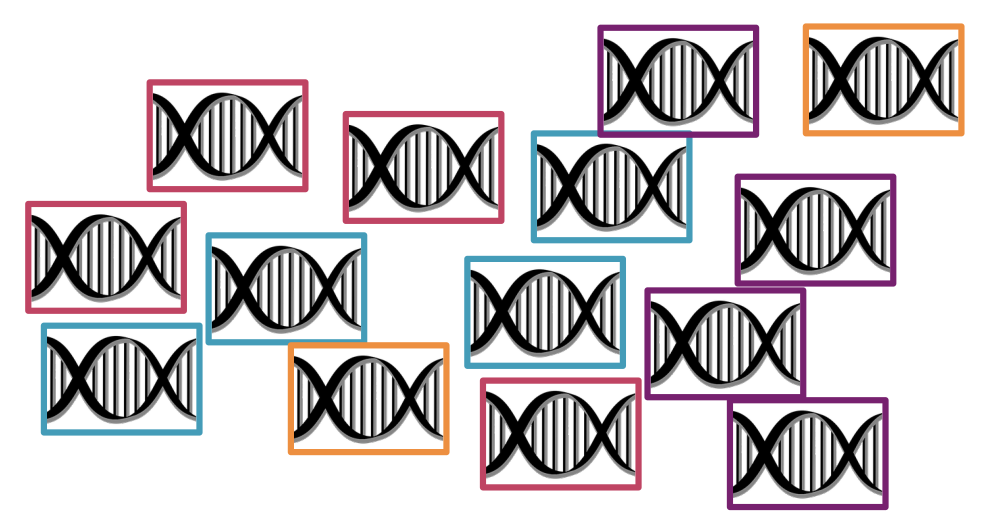
\includegraphics[height=0.5\textheight]{Images/genesGroupes.png}
		
		\vspace*{1em}
		\footnotesize{\textcolor{MPTgrey}{Image tirée d'une présentation donnée par Chloé-Agathe\\ Azencott en 2019 aux Mines de Paris (Fontainebleau)}\\[2.2em]}
	}

		\only<2>{
		\Large \textbf{Segmentation de marché}\\[0.4em]
		\normalsize Permet d'identifier des groupes d’usagers ou de clients dont le \\ comportement est similaire afin de mieux comprendre leur profil\\[0.8em]
		
		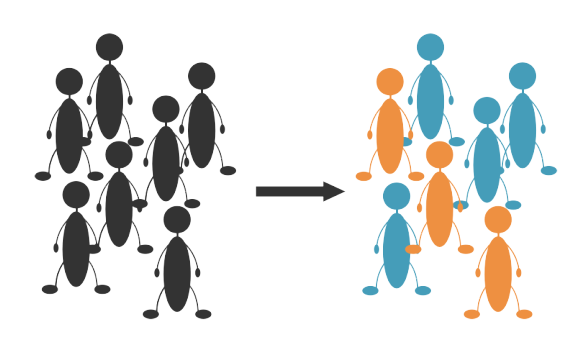
\includegraphics[height=0.5\textheight]{Images/segmentation.png}
		
		\vspace*{0.3em}
		\footnotesize{\textcolor{MPTgrey}{Image tirée d'une présentation donnée par Chloé-Agathe\\ Azencott en 2019 aux Mines de Paris (Fontainebleau)} }	
	}

\only<3>{
	\Large \textbf{Compression d'image}\\[1.5em]
	
	
	\begin{tikzpicture}
		\node (ref) [] {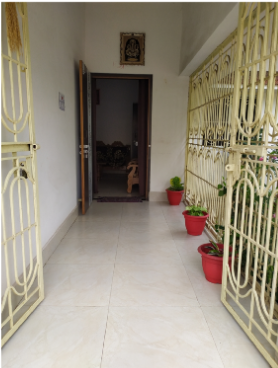
\includegraphics[height=40mm,width=35mm,clip]{Images/compr.png}};
		\node (note)[]  at([yshift = -4]ref.south) {\footnotesize Image originale};
		\node (ref1) [] at([xshift =60]ref.east) {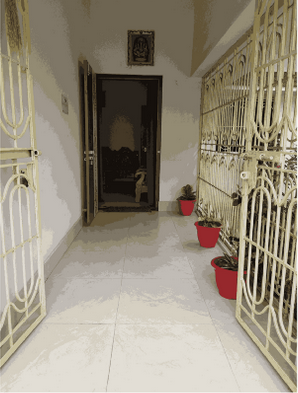
\includegraphics[height=40mm,width=35mm,clip]{Images/compr2.png}};
		\node (note1)[]  at([yshift = -4]ref1.south) {\footnotesize Image compressée (16 couleurs)};
		\node (ref2) at([xshift =60]ref1.east) {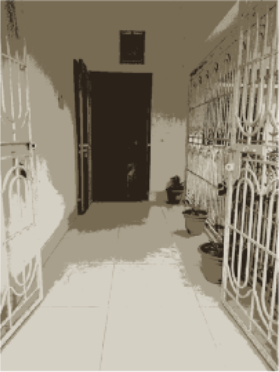
\includegraphics[height=40mm,width=35mm,clip]{Images/compr3.png}};
		\node (note2)[]  at([yshift = -4]ref2.south) {\footnotesize Image compressée (4 couleurs)};
	\end{tikzpicture}
	
	\vspace*{0.3em}
	\footnotesize{\textcolor{MPTgrey}{Image tirée du site \href{https://towardsdatascience.com/image-compression-using-k-means-clustering-aa0c91bb0eeb}{Towards Data Science} }}
	
}

		\only<4>{
	\Large \textbf{Annotation d'un corpus de texte}\\[0.4em]
	\normalsize En regroupant automatiquement l'ensemble des textes par sujet à l'aide d'un algorithme de clustering, il est possible de déterminer le ou les sujets abordés par des textes d'un même cluster en lisant seulement quelques textes de ce cluster\\[0.8em]
	
	
\includegraphics[height=0.5\textheight]{Images/texte.jpg}
	
	\vspace*{0.3em}
\footnotesize{\textcolor{MPTgrey}{Image tirée du site \href{https://fr.dreamstime.com/illustration-stock-remettez-dessin-du-texte-des-graphiques-papier-feuille-image81266457}{Dreamstime} }}	
}


\end{center}
\end{frame}

%------------------------------------------------------------------------------------------
%------------------------------------------------------------------------------------------
\begin{frame}{Choix d'une distance}
		\bftitle{Objectif} \hsp Séparer les données en sous-groupes, appelés \textbf{clusters} tels que\\
		\phantom{\bftitle{Objectif} \hsp} chaque cluster est le plus \textbf{homogène} possible et les clusters entre\\
		\phantom{\bftitle{Objectif} \hsp} eux sont les plus \textbf{distincts}/\textbf{séparés} possible\\[0.8em]
		
\phantom{\bftitle{Objectif} \hsp} On souhaite donc que les individus similaires soient dans le même\\
\phantom{\bftitle{Objectif} \hsp} cluster et que les individus dissimilaires soient dans des clusters\\
\phantom{\bftitle{Objectif} \hsp} différents. \bfblue{Comment mesurer la distance entre deux individus ?} \\

\begin{minipc}[0.17]{0.17}
\hsp \hsp \raisebox{1.5mm}{\bclampe \xspace} 
\end{minipc}
\begin{minipc}[0.75]{0.17}
	On mesure la distance entre deux individus à l'aide d'\textbf{une fonction $d$ appelée distance}
\end{minipc}

		
		\textcolor{MPTblue}{\large\textbf{Définition}}\\
		\vspace*{-0.1em}		
		\begin{vblock}{}
		Soit un ensemble $\X$. Une fonction $d:\X\times\X \to \bbR_+$ est appelée \textit{distance} si elle vérifie les propriétés suivantes :
		
		\vspace*{0.5em}
		\begin{itemize}
			\item[\ex] \,$\forall \ x, y \in \X$ \hsp  \(d(x, y)=d(y, x)\) \hsp \textbf{(Symétrie)}\\[0.5em]
			\item[\ex]  \, $\forall \ x, y \in \X$ \hsp \(d(x, y)=0\Leftrightarrow x=y\) \hsp \textbf{(Séparation)}\\[0.5em]
			\item[\ex]  \, \(\forall \ x, y, z \in \X\) \hsp  \(d(x, y)\leq d(x, z)+d(z, y)\) \hsp \textbf{(Inégalité triangulaire)}
				\end{itemize}
	\end{vblock}
		
\end{frame}

%------------------------------------------------------------------------------------------
%------------------------------------------------------------------------------------------
\begin{frame}{Distances -- variables quantitatives}
	\vspace*{-2em}
	
	\begin{itemize}
		\item  \hsp $x=(x_1,\dots,x_d), y=(y_1,\dots, y_d) \in \bbR^d$ variables \textbf{quantitatives} \hfill $\color{MPTgrey} d \in \bbN^*$\\[2em]
		
		\bftitle{Exemple de distance : }\\[0.8em]
		
		\begin{itemize}
			\normalsize{
			\item[\ex] \hsp \textbf{Euclidienne} \hsp -- \hsp  \(d(x, y)=\lVert x-y\rVert_2 = \sqrt{\sum_{i=1}^d (x_i-y_i)^2}\)\\[0.9em]
			\item[\ex] \hsp \textbf{Manhattan} \hsp -- \hsp \(d(x, y)=\lVert x-y\rVert_1 = \sum_{i=1}^d |x_i-y_i|\)\\[0.9em]
			\item[\ex] \hsp \textbf{Minkowski} \hsp -- \hsp $d(x, y)=\left(\sum_{i=1}^d (x_i-y_i)^p\right)^{1/p}$ \hfill $\color{MPTgrey} p \in \bbR^*$\\[0.9em]
			\item[\ex] \hsp \textbf{Chebyshev} \hsp -- \hsp \(d(x, y)=\max_{i \in \{1,\dots,n\}}|x_i-y_i|\)\\[0.9em]
			\item[\ex] \hsp \textbf{Mahalanobis} \hsp -- \hsp \(d(x, y)=\sqrt{(x-y)^\top \Sigma^{-1}(x-y)}\)  \\[0.2em]
			\phantom{\hsp \textbf{Mahalanobis} \hsp -- \hsp}$ \color{MPTgrey} \Sigma $ \textcolor{MPTgrey}{: matrice de variance-covariance empirique}\\[0.9em]
		%	\item[\ex] \hsp \textbf{Hamming} \hsp -- \hsp \(d(x, y)=\sum_{i=1}^d \mathbb{1}\{x_i\neq y_i\}\)
		}
		\end{itemize}
	\end{itemize}

\vspace*{1em}

\bftitle{Remarque} \hsp On considère souvent la distance euclidienne que l'on notera plus simplement $\| \cdot \|$ par la suite.
\end{frame}
%------------------------------------------------------------------------------------------
%------------------------------------------------------------------------------------------
\begin{frame}{Distances -- variables qualitatives ou mixtes}
	
	\begin{itemize}
		\item  \hsp $x=(x_1,\dots,x_d), y=(y_1,\dots, y_d)$ variables \textbf{qualitatives}\\[2em]
		
		\bftitle{Exemple de distance : } Distance du $\huge \mathbf{\chi_2}$, distance de Jaccard, distance de Gower. 
			\textcolor{MPTgrey}{Ces distances ne sont pas des distances au sens mathématique. La distance du $\color{MPTgrey} \chi_2$ ne respecte par exemple pas la propriété de symétrie}	\\[3em]
		
%		\begin{itemize}
%			\normalsize{
%				\item[\ex] \hsp Distance du $\huge \mathbf{\chi_2}$, distance de Jaccard, distance de Gower.
				% : la plus utilisée en pratique %\hsp -- \hsp  \(d(x, y)=\lVert x-y\rVert_2 = \sqrt{\sum_{i=1}^d (x_i-y_i)^2}\)
%				\\[1em]
				
%				\textcolor{MPTgrey}{Ces distances ne sont pas des distances au sens mathématique. La distance du $\chi_2$ ne respecte par exemple pas la propriété de symétrie}	\\[1em]
%			}
%		\end{itemize}
	
		\item  \hsp $x=(x_1,\dots,x_d), y=(y_1,\dots, y_d)$ variables \textbf{quantitatives et qualitatives}\\[2em]
		
		\bftitle{Exemples de stratégies possibles : }\\[0.8em]
		
		\begin{itemize}
			\normalsize{
								\item[\ex] \hsp Rendre les variables quantitatives qualitatives (découpage en classes)\\[0.9em]
					\item[\ex] \hsp Rendre les variables qualitatives quantitatives (ex : encodage one-hot) \\[0.9em]
\item[\ex] \hsp Rendre toutes les variables qualitatives puis faire une analyse des correspondances multiples (ACM) et considérer les coordonnées (quantitatives) des individus dans les nouveaux axes.\\
			}
		\end{itemize}
	\end{itemize}
	
	
\end{frame}
%------------------------------------------------------------------------------------------
%------------------------------------------------------------------------------------------
\begin{frame}{Choix d'une partition}
\bftitle{Question} \hsp Une fois la distance choisie, quelle partition (clustering) choisir ?\\[2em]


\begin{center}
	
		\begin{tikzpicture}
		%\node (ref) [visible on=<1->] {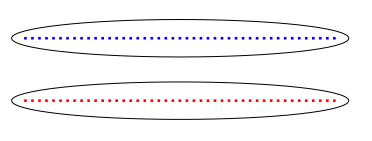
\includegraphics[width=0.35\textwidth,clip]{Images/clusterligne1.png}};
		\node (wiki) at(3,0) [text width=5cm]  {Stratégie de ne pas séparer les points proches l'un de l'autre \textcolor{MPTgrey}{(\eg algorithme de clustering hiérarchique avec lien simple)}};
		%
		%\node (ref1)
		% at([xshift = 6cm]ref)
	%	[right=of ref,visible on=<1->]
	%	{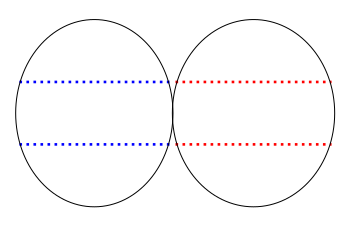
\includegraphics[width=0.35\textwidth,clip]{Images/clusterligne2.png}};
		\node (wiki1)[text width=5.4cm] at([xshift = 6cm]wiki) {Stratégie de ne pas avoir des points trop éloignés dans le même cluster \textcolor{MPTgrey}{(\eg algorithme des 2-moyennes) \phantom{rrrrrrrr}}};		
	\end{tikzpicture}
\vspace*{-1em}

	\begin{tikzpicture}
		\node (ref) [visible on=<1->] {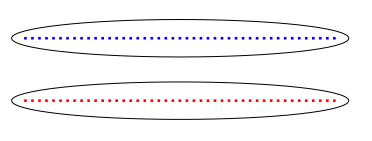
\includegraphics[width=0.35\textwidth,clip]{Images/clusterligne1.png}};
		%\node (wiki)[text width=5cm]   at([yshift = 13]ref.north) {Stratégie de ne pas séparer \newline les points proches (\eg algorithme de clustering hiérarchique avec lien simple)};
		%
		\node (ref1)
		% at([xshift = 6cm]ref)
		[right=of ref,visible on=<1->]
		{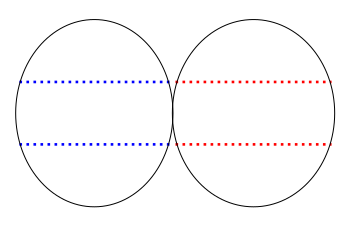
\includegraphics[width=0.35\textwidth,clip]{Images/clusterligne2.png}};
		%\node (wiki)[text width=5cm] at([yshift = 17.5]ref1.north) {Stratégie de ne pas avoir des points trop éloignés dans le même cluster (\eg algorithme des $2$-moyennes)};		
	\end{tikzpicture}
	
	\footnotesize{\textcolor{MPTgrey}{Tirée de l'ouvrage \textit{\href{https://www.cs.huji.ac.il/~shais/UnderstandingMachineLearning/understanding-machine-learning-theory-algorithms.pdf}{Understanding Machine Learning: From Theory to Algorithms}}} }
\end{center}

\begin{minipc}[0.13]{0.15}
	\raisebox{1.5mm}{\bclampe \xspace} 
\end{minipc}
\begin{minipc}[0.75]{0.15}
On voudrait choisir la partition qui minimise un certain critère (à choisir) qui dépend de l'homogénéité et de la séparabilité des clusters  
\end{minipc}	
	
	
\end{frame}
%------------------------------------------------------------------------------------------
%------------------------------------------------------------------------------------------
\begin{frame}{Homogénéité}
				\vspace*{-0.7em}
	\only<1>{
	Le fait que des observations proches appartiennent au même cluster peut se traduire par la notion d’homogénéité\\[0.5em]
			\textcolor{MPTblue}{\large\textbf{Définition}}\\
	\vspace*{-0.1em}		
	\begin{vblock}{}
	On appelle \textit{centroïde} du cluster $\C$ le point défini par 
		\vspace*{-0.5em}
	$$\mu_{\C} = \dfrac{1}{\vert \C \vert}\sum_{x \in \C} x \hsp \hsp \vert \C\vert :  \text{ nombre d'observations dans } \C $$
			\vspace*{-1.3em}
%	avec $\vert \C\vert$ le nombre d'observations dans $\C$ 
	\end{vblock}

		\vspace*{-0.5em}		
	\textcolor{MPTblue}{\large\textbf{Définition}}\\
	\vspace*{-0.1em}		
	\begin{vblock}{}
		On appelle \textit{homogénéité} du cluster $\C_k$ (\textit{tightness} en anglais) la moyenne des distances des observations de ce cluster à son centroïde $\mu_k$ :
		\vspace*{-0.5em}
	$$ T_k= \dfrac{1}{\vert \C_k \vert} \sum_{x \in \C_k} d(x, \mu_k)  $$	
L’\textit{homogénéité globale} d’un clustering de $\D$ de taille $K$ est donné par\\[0.5em]
\phantom{a}\hfill $ T= \frac{1}{K} \sum_{k=1}^K T_k$ \hfill \phantom{a}
	%\vspace*{-1.3em}
	\end{vblock}

	\vspace*{-0.9em}
\bftitle{Remarque} \hsp On souhaite avoir $T$ le plus petit possible\\[1em]
}
\only<2>{
	
		\begin{center}
		
		
		
		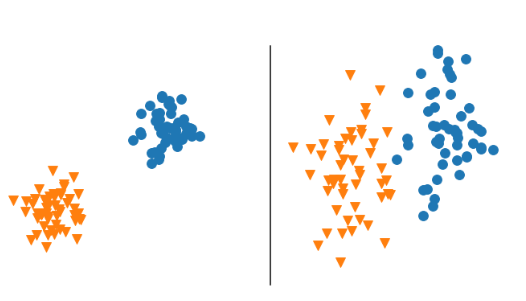
\includegraphics[width=0.9\textwidth]{Images/homogene.png}
		
		\vspace*{0.5em}
		\footnotesize{\textcolor{MPTgrey}{Tirée de l'ouvrage \textit{\href{http://cazencott.info/dotclear/public/lectures/IntroML_Azencott.pdf}{Introduction au Machine Learning}} de Chloé-Agathe Azencott} }
	\end{center}

}	
\end{frame}
%------------------------------------------------------------------------------------------
%------------------------------------------------------------------------------------------
\begin{frame}{Séparabilité}
	\only<1>{
Pour quantifier à quel point les clusters sont distants les uns des autres, nous pouvons utiliser le critère de séparabilité\\[2em]

	%			
	\textcolor{MPTblue}{\large\textbf{Définition}}\\
	\vspace*{-0.1em}		
	\begin{vblock}{}
		On appelle \textit{séparabilité} des clusters $\C_k$ et $\C_\ell$ la distance entre leurs centroïdes :
		$$ S_{k\ell}= d(\mu_k, \mu_\ell)  $$
		La \textit{séparabilité globale} d’un clustering de $\D$ de taille $K$ se calcule comme la moyenne des séparabilités des clusters deux à deux :
		$$ S = \dfrac{2}{K(K-1)} \sum_{k=1}^K \sum_{\ell=k+1}^K \, S_{k\ell}$$	
		\vspace*{-1.2em}
	\end{vblock}
	
		\vspace*{1em}
	\bftitle{Remarque} \hsp On souhaite avoir $S$ le plus élevé possible\\[1em]
}
\only<2>{
	
	\begin{center}
		
		
		
		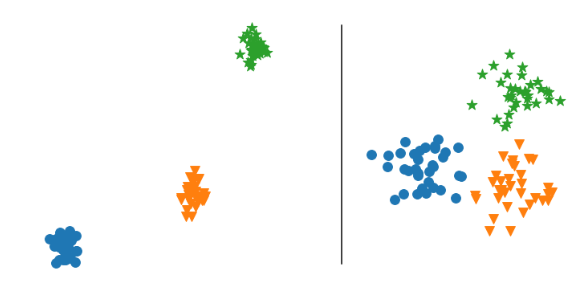
\includegraphics[width=0.9\textwidth]{Images/separabilite.png}
		
		\vspace*{0.5em}
		\footnotesize{\textcolor{MPTgrey}{Tirée de l'ouvrage \textit{\href{http://cazencott.info/dotclear/public/lectures/IntroML_Azencott.pdf}{Introduction au Machine Learning}} de Chloé-Agathe Azencott} }
	\end{center}
	
}	
\end{frame}
%------------------------------------------------------------------------------------------
%------------------------------------------------------------------------------------------
\begin{frame}{Indice de Davies-Bouldin}
	
		\textcolor{MPTblue}{\large\textbf{Définition}}\\
	\vspace*{-0.1em}		
	\begin{vblock}{}
		On appelle \textit{indice de Davies-Bouldin} du cluster $\C_k$ la valeur
		$$ D_{k}= \underset{\ell\neq k}{\max} \, \dfrac{T_k + T_\ell}{S_{k\ell}} $$
		Cela revient donc à regarder le "pire des cas" en termes d'homogénéité et de séparabilité\\[1em]
		L'\textit{indice de Davies-Bouldin global} d’un clustering de $\D$ de taille $K$ se calcule comme la moyenne des indices de  Davies-Bouldin des clusters :
		$$ D = \dfrac{1}{K}\sum_{k=1}^K D_k$$	
		\vspace*{-1.2em}
	\end{vblock}

\vspace*{1em}

\bftitle{Objectif} \hsp On souhaite trouver le clustering $\D$ qui minimise $D$\\[1em]
	
\end{frame}
%------------------------------------------------------------------------------------------
%------------------------------------------------------------------------------------------
\begin{frame}{Coefficient de silhouette}
		\vspace*{-0.5em}
	\begin{minipt}[1]{0.79}
			\textcolor{MPTblue}{\large\textbf{Définition}}\\
	\vspace*{-1.2em}		
	\begin{vblock}{}
		On appelle \textbf{coefficient de silhouette} de l'observation $x \in \{x_1,\dots,x_n\}$ la valeur
		$$ s(x)= \dfrac{b(x)-a(x)}{\max(\left(a(x), b(x)\right)} \, \in [-1,1]$$
		\vspace*{-0.5em}
$$\text{avec} \hspace*{2em} a(x) = \dfrac{1}{\vert\C_{k(x)}\vert - 1}  \sum_{y\in \C_{k(x)}, y \neq x} d(x,y) \hspace*{2em} b(x) = \underset{\ell\neq k(x)}{\min} \dfrac{1}{\vert\C_\ell\vert}  \sum_{y\in \C_{\ell}} d(x,y)$$
		\ie $a(x)$ est la distance moyenne de $x$ à tous les autres éléments du cluster $\C_{k(x)}$ auquel il appartient et $b(x)$ est la plus petite valeur que pourrait prendre $a(x)$ si $x$ appartenait à un autre cluster\\[0.5em]
		
			\vspace*{-.5em}
		Le \textit{coefficient de silhouette global} se calcule comme la moyenne des coefficients de silhouette :
		$$ s = \dfrac{1}{n}\sum_{i=1}^n s(x_i)$$
	

		\vspace*{-1.2em}
	\end{vblock}
\end{minipt}
\begin{minipt}[1]{0.1}

	\only<1>{
			\vspace*{-0.4em}
\bftitle{Remarque} \hsp Le coefficient de silhouette de $x$ est d’autant plus proche de 1 que\\\phantom{\bftitle{Remarque} \hsp} son assignation au cluster $\C_{k(x)}$ est satisfaisante 
}
	\only<2>{
\bftitle{Objectif} \hsp On souhaite trouver le clustering $\D$ qui maximise $s$
}
\end{minipt}
\note{faire un dessins pour expliquer avec deux clusters et demander comment on change le dessin pour que  $b(x)$ soit plus grand}
\end{frame}
%------------------------------------------------------------------------------------------
%------------------------------------------------------------------------------------------
\begin{frame}{Inertie intra et inter classes}
		\vspace{-0.5em}
	\bftitle{Contexte} \hsp On observe des \textbf{données} $x_1,\dots,x_n \in \bbR^d$. On note $\mu = \frac{1}{n} \sum_{i=1}^n x_i$\\[-0.1em]
	\phantom{\bftitle{Contexte} \hsp} et on considère la distance euclidienne\\[1.5em]
	
On peut également quantifier la notion d'homogénéité et de séparabilité d'un clustering $\D$ de taille $K$ de $\{x_1,\dots,x_n\}$ à travers la notion d'inertie donnée par 
	\vspace{-0.5em}
	$$ I = \sum_{i =1}^n \| x_i - \mu \|^2 = \sum_{k =1}^K \sum_{x_i \in \C_k} \|x_i - \mu_k \|^2  + \sum_{k =1}^K \vert C_k \vert \, \| \mu_k - \mu \|^2$$
	
Aussi, $I$ se décompose en deux parties :\\[0.5em]
\begin{itemize}
	\item $I_W = \sum_{k =1}^K \sum_{i \in \C_k} \|x_i - \mu_k \|^2 $  : \textbf{inertie intra-classes} qui mesure l'homogénéité au sein des classes\\[0.5em]
	\item $I_B = \sum_{k =1}^K \vert \C_k \vert \, \| \mu_k - \mu \|^2$ : \textbf{inertie inter-classes} qui mesure l'hétérogénéité entre les classes, c'est-à-dire à quel point les classes sont bien séparées\\[1.5em]
\end{itemize}	

\bftitle{Objectif} \hsp On souhaite trouver le clustering $\D$ qui maximise $I_B$ ou de manière\\
\phantom{\bftitle{Objectif} \hsp} équivalente qui minimise $I_W$
	
%\bftitle{Remarque} \hsp On peut également quantifier la notion d'homogénéité et de\\
%\phantom{\bftitle{Remarque} \hsp} séparabilité d'un clustering $\D$ de taille $K$ de $\{xi,\dots,x_n\}$ à\\
%\phantom{\bftitle{Remarque} \hsp} travers la notion d'inertie, notée $I$

	\note{Ici on peut dire que cette slide met en avant le fait qu'il y ait un jeu entre homogénéité et séparabilité pas mis en avant avant. En effet, pour avoir des clusters homogènes, on pourrait faire des petits groupes. Mais alors on diminuerait la séparabilité. Leur demander pourquoi ? imaginer un cas de figure.
	
	Aussi : demander pourquoi dans inter inter classes : on pndère par $\vert \C_k \vert$ :parce qu'on veut prendre en compte la taille du cluster }
\end{frame}
%------------------------------------------------------------------------------------------
%------------------------------------------------------------------------------------------
%------------------------------------------------------------------------------------------
%------------------------------------------------------------------------------------------
\begin{frame}{Choix d'une partition}
	
	\bftitle{Contexte} \hsp On souhaite partitionner des \textbf{données} $x_1,\dots,x_n \in \X$ \\[0.5em]
	
	\begin{minipc}[0.08]{0.15}
		\raisebox{1.5mm}{\bclampe \xspace} 
	\end{minipc}
	\begin{minipc}[0.9]{0.15}
		On voudrait choisir la partition $\C^*$ qui minimise un certain critère $R$ (à choisir) qui dépend de l'homogénéité et de la séparabilité des clusters  
	\end{minipc}	
	
	$$ \C^* = \underset{K \in \{1,\dots, n\}}{\text{arg}\,\min}\,\,\underset{\C_1,\dots,\C_K}{\min}\,\, R(\C_1,\dots,\C_K)$$

avec $R(\C_1,\dots,\C_K)$ l’indice de Davies-Bouldin global, le coefficient de silhouette global ou la variance intra-classes du clustering $\D=\{\C_1,\dots,\C_K\}$\\[1em]

	\begin{minipc}[0.08]{0.15}
	\warning
\end{minipc}
\begin{minipc}[0.9]{0.15}
	Le nombre de partitions possibles $B_n$, appelé nombre de Bell, est trop grand~; on ne peut pas explorer toutes les possibilités :
	\end{minipc}
%	\vspace{-1.5em}
$ \phantom{a} \hfill \hsp \hsp \hsp \hsp B_n = \dfrac{1}{e} \sum_{K\geq1} \dfrac{K^n}{K !}\hfill \phantom{a}$ \hfill $\color{MPTgrey}B_{50}\geq 10^{48}$


	\begin{minipc}[0.08]{0.15}
	\raisebox{1.5mm}{\bclampe \xspace} 
\end{minipc}
\begin{minipc}[0.9]{0.15}
	On va utiliser des algorithmes itératifs qui visent à explorer un sous
	ensemble de partitions dans lequel on espère que se trouve la
	partition optimale
\end{minipc}
\end{frame}
%------------------------------------------------------------------------------------------
%------------------------------------------------------------------------------------------
\begin{frame}{Stratégie itératives}
	
Différents algorithmes itératifs existent dont les plus courants :\\[2em]

\begin{itemize}
	\item  \hsp les algorithmes agglomératifs ou divisifs : \only<1>{la classification hiérarchique} \only<2>{\textbf{\textcolor{MPTblue}{la classification hiérarchique}}}\\[2em]
		\item  \hsp les algorithmes par partitionnement : \eg \only<1>{les $K$-moyennes} \only<2>{\textbf{\textcolor{MPTblue}{les $\color{MPTblue} K$-moyennes}}}\\[2em]
			\item  \hsp les algorithmes probabilistes : les modèles de mélange\\[2em]
\end{itemize}
	
\end{frame}
%------------------------------------------------------------------------------------------
%------------------------------------------------------------------------------------------

\section{Clustering hiérarchique}
%------------------------------------------------------------------------------------------
%------------------------------------------------------------------------------------------
\begin{frame}{Principe}
	\vspace*{-0,4em}
Le clustering hiérarchique est un algorithme itératif qui propose une partition des données $\{x_1,\dots,x_n\}$ pour toute taille $k \in \{1,\dots,n\}$ possible de partition. Cet algorithme fonctionne par récurrence : chaque nouvelle partition est obtenue à partir de l'ancienne partition.\\[0.9em]

\bftitle{Deux stratégies}\\[0.5em]

\begin{itemize}
	\item \textbf{Clustering agglomératif} : initialement, chaque observation forme un cluster de taille $1$. À chaque itération de l’algorithme, on trouve
	les deux clusters les plus proches, et on les agglomère en un seul cluster, et ce jusqu’à ne plus avoir qu’un	unique cluster contenant les $n$ observations.\\[1em]
	\item \textbf{Clustering divisif} : initialement, toutes les observations sont dans un même cluster de taille $n$. À chaque itération, on sépare un cluster en deux jusqu’à ce que chaque cluster ne contienne plus qu’une seule observation.\\[0.9em]
\end{itemize}
\begin{valblock}{}
	Par la suite, on s'intéresse au \textbf{clustering agglomératif} aussi appelé \textbf{classification ascendante hiérarchique} (CAH)
	\end{valblock}

\vspace*{-0.5em}
\bftitle{Question} \hsp Comment mesurer la distance entre deux clusters ?\\[1em]
\end{frame}
%------------------------------------------------------------------------------------------
%------------------------------------------------------------------------------------------
\begin{frame}{Distance entre deux clusters}	
	\vspace*{-0.7em}
	Soit $\C_k$, $C_\ell$ deux clusters\\[0.3em]
	
	\bftitle{Exemples de distance/dissimilarité entre $\color{MPTblue} \C_k$ et $\color{MPTblue} C_\ell$} \\[0.3em]	
	\begin{itemize}
		\item[\ex] \textbf{lien simple} : $d(\C_k$, $\C_\ell) = \underset{(x,y) \in \C_k \times \C_\ell}{\min} d(x,y)$\\[0.1em]
		$ \C_k$ et $C_\ell$ sont agglomérés si deux de leurs éléments sont proches\\[1em]
		\item[\ex] \textbf{lien complet} : $d(\C_k$, $\C_\ell) = \underset{(x,y) \in \C_k \times \C_\ell}{\max} d(x,y)$\\[0.1em]
		$ \C_k$ et $\C_\ell$ sont agglomérés si tous leurs éléments sont proches.\\[1em]
		\item[\ex] \textbf{lien moyen} : $d(\C_k$, $\C_\ell) = \dfrac{1}{\vert\C_k\vert}\dfrac{1}{\vert\C_\ell\vert}\sum_{x\in \C_k} \sum_{y \in \C_\ell} d(x,y)$\\[0.1em]
		$ \C_k$ et $\C_\ell$ sont agglomérés si la distance moyenne entre un élément de $ \C_k$ et un élément de $\C_\ell$ est faible.\\[1em]
		\item[\ex] \textbf{lien centroïdal} : $d(\C_k$, $\C_\ell) =  d(\mu_k, \mu_\ell)$\\[0.1em]
		$ \C_k$ et $\C_\ell$ sont agglomérés si la distance entre leurs centroïdes est faible\\[1em]
	\end{itemize}
\bftitle{Remarque} \hsp Ces distances s’attachent à garantir la séparabilité des clusters. Ce ne sont pas forcément des distances au sens mathématique. Par exemple, pour le lien complet $d(\C_k$, $\C_k) \neq 0$ si $|\C_k| >1$
\end{frame}
%------------------------------------------------------------------------------------------
%------------------------------------------------------------------------------------------
\begin{frame}{Distance entre deux clusters}	
	\vspace*{-0.5em}
	Soit $\C_k$, $C_\ell$ deux clusters\\[1em]
	
	\bftitle{Exemples de distance/dissimilarité entre $\color{MPTblue} \C_k$ et $\color{MPTblue} C_\ell$} \\[0.8em]	
	\begin{itemize}
		\item[\ex] \textbf{distance de Ward} : $d(\C_k$, $C_\ell) = \dfrac{\vert \C_k\vert \, \vert \C_\ell\vert}{\vert \C_k\vert + \vert \C_\ell\vert} \| \mu_k - \mu_\ell\|^2$\\[0.5em]
		
\end{itemize}	
	\textcolor{MPTred}{\large\textbf{Proposition}} \hfill $\color{MPTgrey} K \in \{1,\dots , n\}$\\ 
	\vspace*{-0.2em}		
	\begin{valblock}{}
La distance de Ward $d(\C_k$, $C_\ell)$ correspond au gain de variance intra-classe (de manière équivalente, à la perte d’inertie
inter-classes) lorsque l’on fusionne les classes $\C_k$ et $C_\ell$ pour passer de $K$ à $K-1$ classes
	\end{valblock}	
	
	Ainsi, $ \C_k$ et $C_\ell$ sont agglomérés si la fusion de ces deux clusters minimise le gain de variance intra-classe de la nouvelle partition : on maximise l'homogénéité \\[1.5em]
	

	\vspace*{0.2em}
	\bftitle{Remarque} \hsp La distance de Ward maximise aussi la séparabilité entre les\\
	\phantom{\bftitle{Remarque} \hsp} clusters puisqu'elle minimise la perte de variance inter-classe \\[0.8em]
%	\bftitle{Remarque} \hsp La distance de Ward prend en compte les effectifs des groupes : \phantom{\bftitle{Remarque} \hsp} création de groupes équilibrés. \clrcite{Pourquoi ?}
\end{frame}
%------------------------------------------------------------------------------------------
%------------------------------------------------------------------------------------------
\begin{frame}{Distance entre deux clusters}	
	\bftitle{Remarque} \hsp La distance de Ward prend en compte les effectifs des groupes : \phantom{\bftitle{Remarque} \hsp} création de groupes équilibrés. \clrcite{Pourquoi ?}\\[2em]
	
	
	\begin{center}
		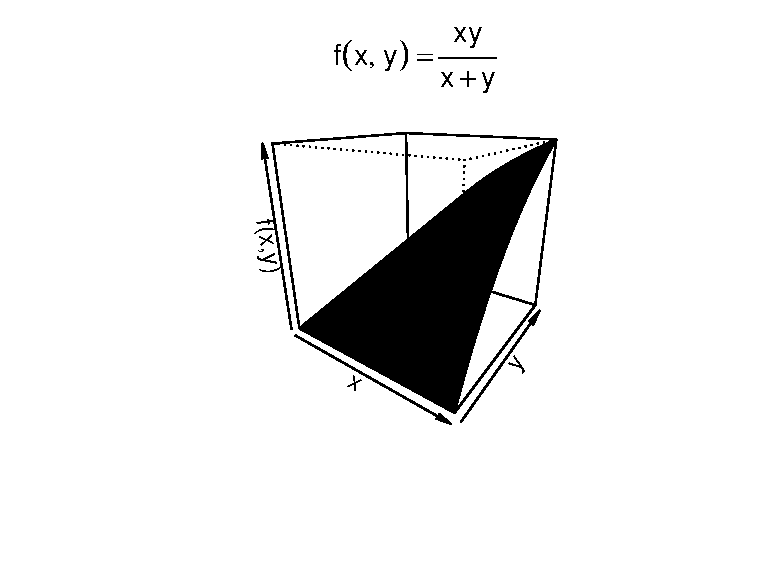
\includegraphics[width=0.8\textwidth]{Images/distWald.pdf}
		
%		\vspace*{0.5em}
%		\footnotesize{\textcolor{MPTgrey}{Tirée de l'ouvrage \textit{\href{http://cazencott.info/dotclear/public/lectures/IntroML_Azencott.pdf}{Introduction au Machine Learning}} de Chloé-Agathe Azencott} }	
	\end{center}
	
\end{frame}

%------------------------------------------------------------------------------------------
%------------------------------------------------------------------------------------------


\begin{frame}{Dendogramme}
Le résultat d’un clustering hiérarchique (agglomératif ou divisif) peut se visualiser sous la forme d’un \textbf{dendrogramme}\\[1em]

\begin{center}
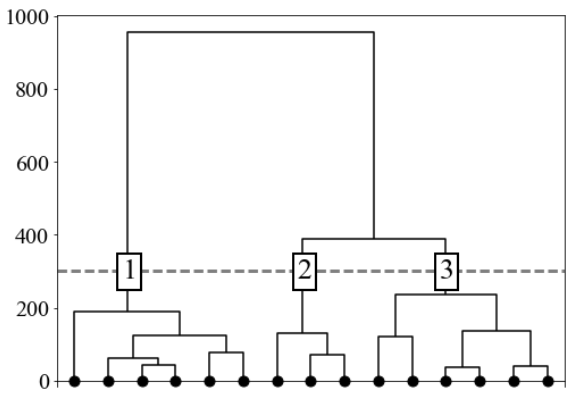
\includegraphics[width=0.6\textwidth]{Images/dendogramme.png}

\vspace*{0.5em}
\footnotesize{\textcolor{MPTgrey}{Tirée de l'ouvrage \textit{\href{http://cazencott.info/dotclear/public/lectures/IntroML_Azencott.pdf}{Introduction au Machine Learning}} de Chloé-Agathe Azencott} }	
\end{center}
	
\bftitle{Remarque} \hsp La longueur d’une branche de l’arbre est égale à la\\ \phantom{\bftitle{Remarque} \hsp} distance entre les deux clusters qu’elle connecte
\end{frame}
%------------------------------------------------------------------------------------------
%------------------------------------------------------------------------------------------
\begin{frame}{Choix du nombre de clusters}
		\vspace*{-0.6em}
L’un des atouts du clustering hiérarchique est qu’il ne requiert pas de spécifier au préalable le nombre de groupes. Le dendrogramme permet d’explorer l’ensemble des partitions envisageables. Toutefois, il reste indispensable, à un moment donné, de déterminer le nombre de clusters retenus\\[0.8em]

Il y a différentes manières de choisir le nombre de clusters :\\[0.8em]

\begin{itemize}
	\item On arrête de fusionner des clusters dès que la distance minimale entre \\les clusters dépasse une certain seuil $r \in \bbR^*$. Ce seuil peut-être choisi arbitrairement ou égal à $\underset{(x,y) \in \{x_1,\dots,x_n\}}{\max}\alpha d(x,y)$ avec $\alpha <1$. \\[0.1em] On peut aussi faire cela visuellement en coupant le dendogramme avant qu'une branche ne soit trop grande\\[0.5em]
	\item On peut évaluer les différentes partitions trouvées, c’est-à-dire les différents nœuds du dendrogramme, à l’aide d’une mesure de performance, \eg le coefficient de silhouette, et choisir la partition avec la meilleure performance\\[1em]
	
\end{itemize}

	\begin{minipc}[0.06]{0.15}
	\warning
\end{minipc}
\begin{minipc}[0.92]{0.15}
La complexité algorithmique du clustering hiérarchique est élevée : à chaque itération, pour décider quels clusters regrouper, il faut calculer les distances deux à deux entre toutes les paires possibles de $\{x_1,\dots,x_n\}$ : $\color{black}O(dn^2)$ opérations
\end{minipc}
%\bftitle{Remarque} \hsp La complexité algorithmique du clustering hiérarchique est élevée :\\ \phantom{\bftitle{Remarque} \hsp} à chaque itération, pour décider quels clusters regrouper, il faut\\ \phantom{\bftitle{Remarque} \hsp} calculer les distances deux à deux entre toutes les paires possibles\\ \phantom{\bftitle{Remarque} \hsp} de $\{x_1,\dots,x_n\}$
\note{expliquer pourquoi c'est $O(dn^2)$ : le $n^2$ vient de choisir deux éléments parmi $n$.}
\end{frame}

%------------------------------------------------------------------------------------------
%------------------------------------------------------------------------------------------

\section{Les $\color{MPTblue}K$-moyennes}
%------------------------------------------------------------------------------------------
%------------------------------------------------------------------------------------------
\begin{frame}{Principe}
	
	\begin{minipc}[0.1]{0.15}
		%\begin{center}
		\raisebox{1.5mm}{\bclampe \xspace} 
	\end{minipc}
	\begin{minipc}[0.89]{0.15}
	Plutôt que d’explorer toutes les tailles de partition possibles il peut être préférable de se fixer un nombre $K$ de clusters au préalable, ce qui permet de réduire les temps de calculs.
		\end{minipc}
	
	\vspace*{2em}
	\bftitle{Objectif} \hsp Pour $K$ fixé, trouver
	la partition de taille $K$  des données $\{x_1,\dots,x_n\}$\\
	\phantom{\bftitle{Objectif} \hsp} qui minimise l'inertie intra-classes : 
	$$ \C^* =  \underset{\C_1,\dots,\C_K}{\text{arg}\,\min} \sum_{k=1}^K \sum_{x \in \C_k} \|x-\mu_k\|^2$$
	
	\vspace*{1em}
		\begin{minipc}[0.1]{0.1}
		\warning
	\end{minipc}
	\begin{minipc}[0.89]{0.1}
Problème d'optimisation trop long à résoudre
	\end{minipc}
	\begin{minipc}[0.1]{0.1}
	%\begin{center}
	\raisebox{1.5mm}{\bclampe \xspace} 
\end{minipc}
\begin{minipc}[0.89]{0.1}
Utiliser une heuristique : \textit{l’algorithme de Lloyd}
\end{minipc}
\end{frame}
%------------------------------------------------------------------------------------------

\begin{frame}{Algorithme de Lloyd}

\only<1>{	
	\begin{enumerate}
		\item Choisir $K$ observations $\mu_1,\dots \mu_K$ aléatoirement dans l'espace pour servir de centroïdes initiaux. On les choisit en général parmi les points de données de manière aléatoire alors de sorte à les disperser au maximum parmi les données~: \textit{algorithme K-means++} (mais ça pourrait être aussi des points choisies aléatoires dans l'espace). 
			%On peut également les choisir aléatoirement dans $\X$ : c'est ce qui est fait en pratique
			\\[2em]
		\item Affecter chaque observation $x_i$ au centroïde dont elle est le plus proche :
		$$ k(x_i) = \underset{k=1,\dots,K}{\text{arg}\,\min} \|x_i-\mu_k\|^2$$
		
		\vspace*{-1em}
		Cela revient à regarder dans quelle cellule du diagramme de Voronoï induit par $\mu_1,\dots \mu_K$ le point $x_i$ se trouve\\[2em] 
		\item Recalculer les centroïdes de chaque cluster : 
		$ \mu_k = \dfrac{1}{\vert C_k\vert}\sum_{x_i \in \C_k} x_i$\\[2em]
		\item Répéter les opérations 2–3 jusqu’à convergence, c’est-à-dire jusqu’à ce que les affectations ne changent plus
	\end{enumerate}
}
\end{frame}
%------------------------------------------------------------------------------------------
\begin{frame}{Algorithme de Lloyd}
	
	\begin{center}
		Voir  \href{https://en.wikipedia.org/wiki/K-means_clustering\#/media/File:K-means_convergence.gif}{cette animation}
	\end{center}	
\end{frame}
%------------------------------------------------------------------------------------------	

\begin{frame}{Algorithme de Lloyd - variante}

	\vspace*{-1em}
	\begin{center}
		
		\begin{tikzpicture}
			\node (ref) [visible on=<1>] {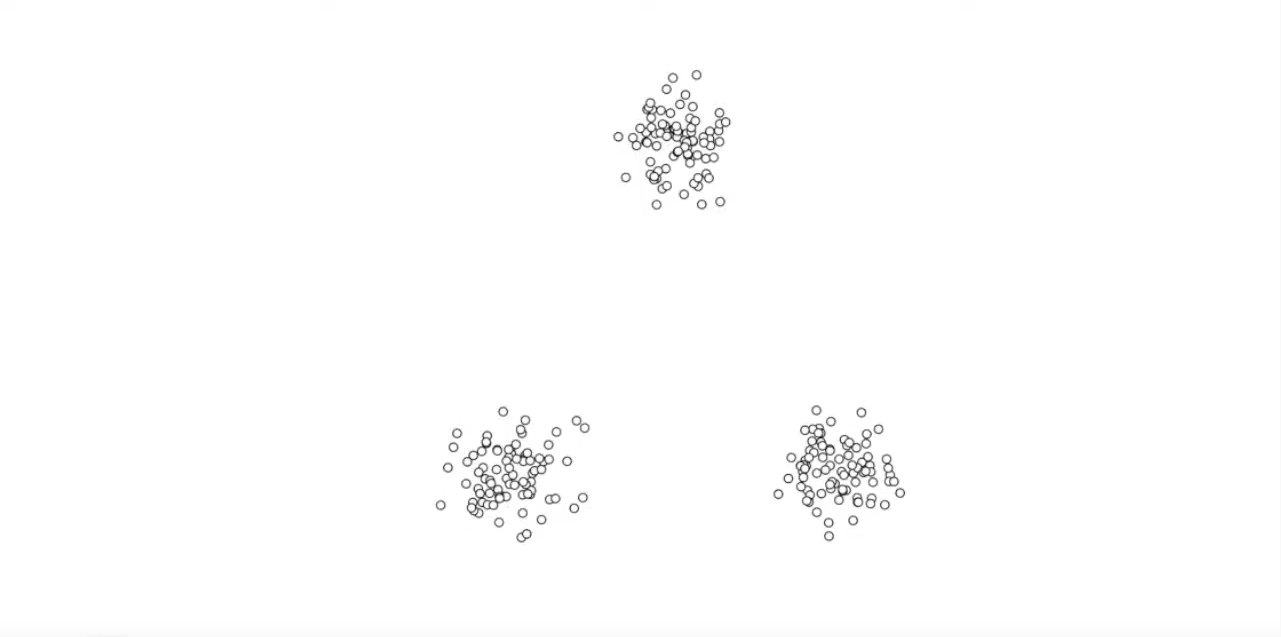
\includegraphics[width=0.99\textwidth,clip]{kmeans1.png}};
			\node (wiki)[visible on=<1>]  at([yshift = 13]ref.north) {Données};
			%
			\node (ref) [visible on=<2>] {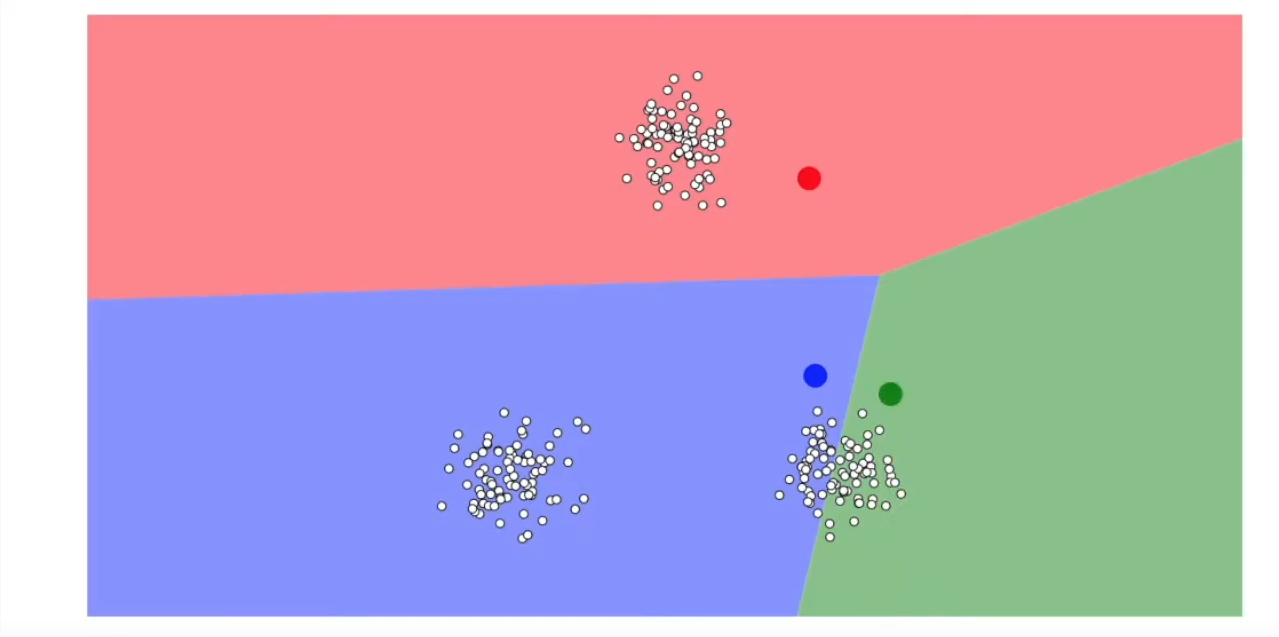
\includegraphics[width=0.99\textwidth,clip]{kmeans2.png}};
			\node (wiki)[visible on=<2>,text width=11cm]  at([yshift = 18]ref.north) {\hsp \, \, Choix des centroïdes $\mu_1,\mu_2,\mu_3$ \hsp \, \,  (nombre de clusters $K=3$)  \hsp 
				  \footnotesize \, ici, les centroïdes de départ ne correspondent pas à des données
			};
			%
			\node (ref) [visible on=<3>] {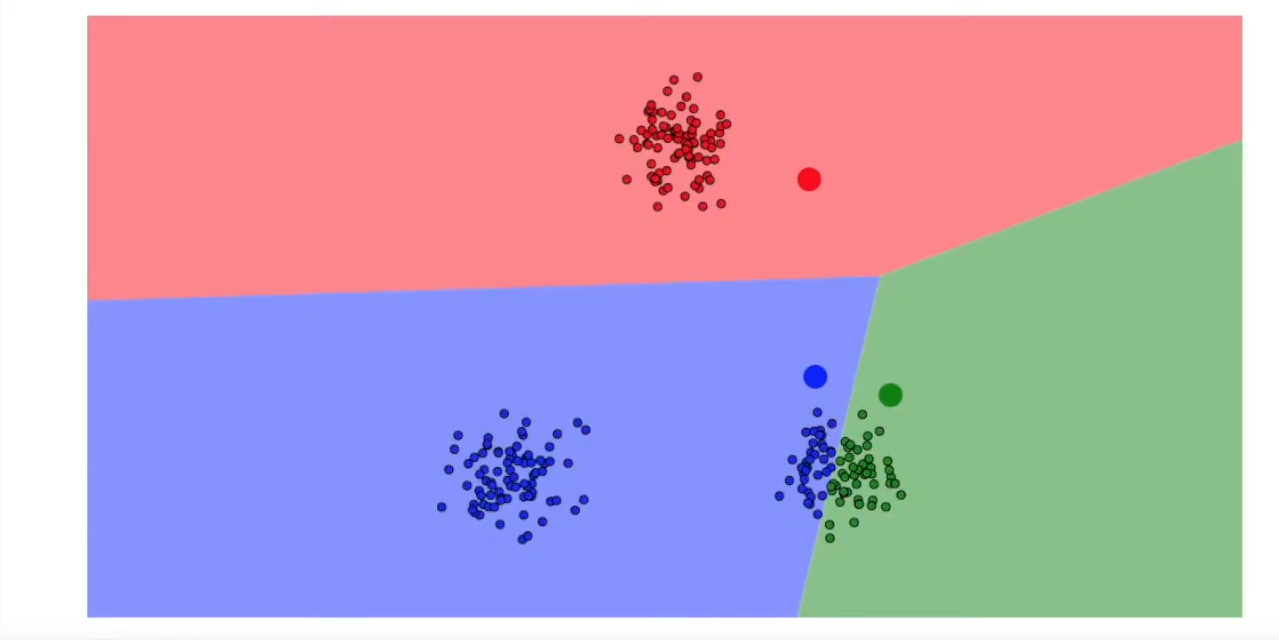
\includegraphics[width=0.99\textwidth,clip]{kmeans3.png}};
			\node (wiki)[visible on=<3>]  at([yshift = 13]ref.north) {Affectation des données au centroïde le plus proche};
			%
			\node (ref) [visible on=<4>] {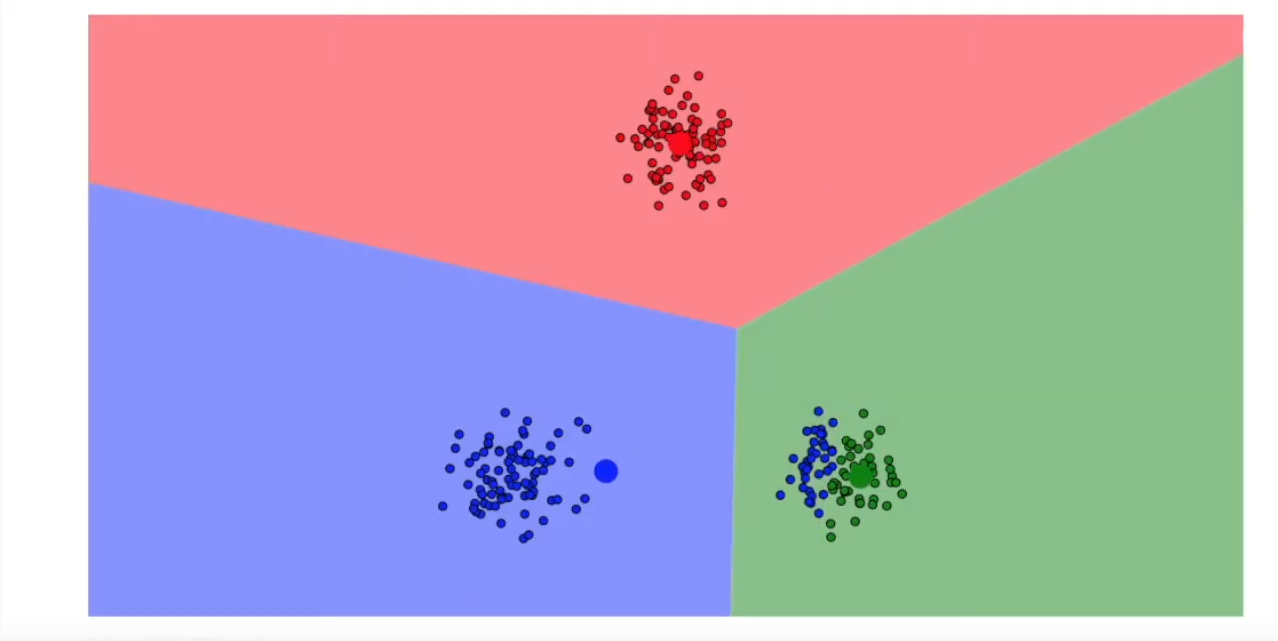
\includegraphics[width=0.99\textwidth,clip]{kmeans4.png}};
			\node (wiki)[visible on=<4>]  at([yshift = 13]ref.north) {Recalcul des centroïdes};
			%
			\node (ref) [visible on=<5>] {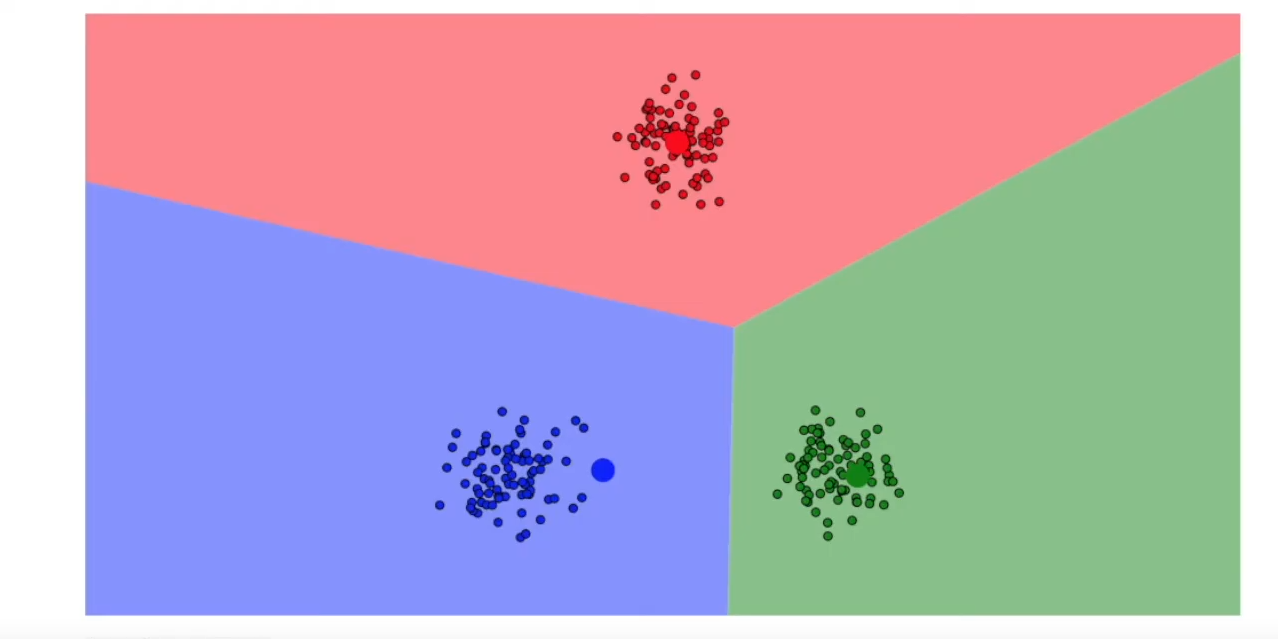
\includegraphics[width=0.99\textwidth,clip]{kmeans5.png}};
			\node (wiki)[visible on=<5>]  at([yshift = 13]ref.north) {Affectation des données au centroïde le plus proche};
			%
			\node (ref) [visible on=<6>] {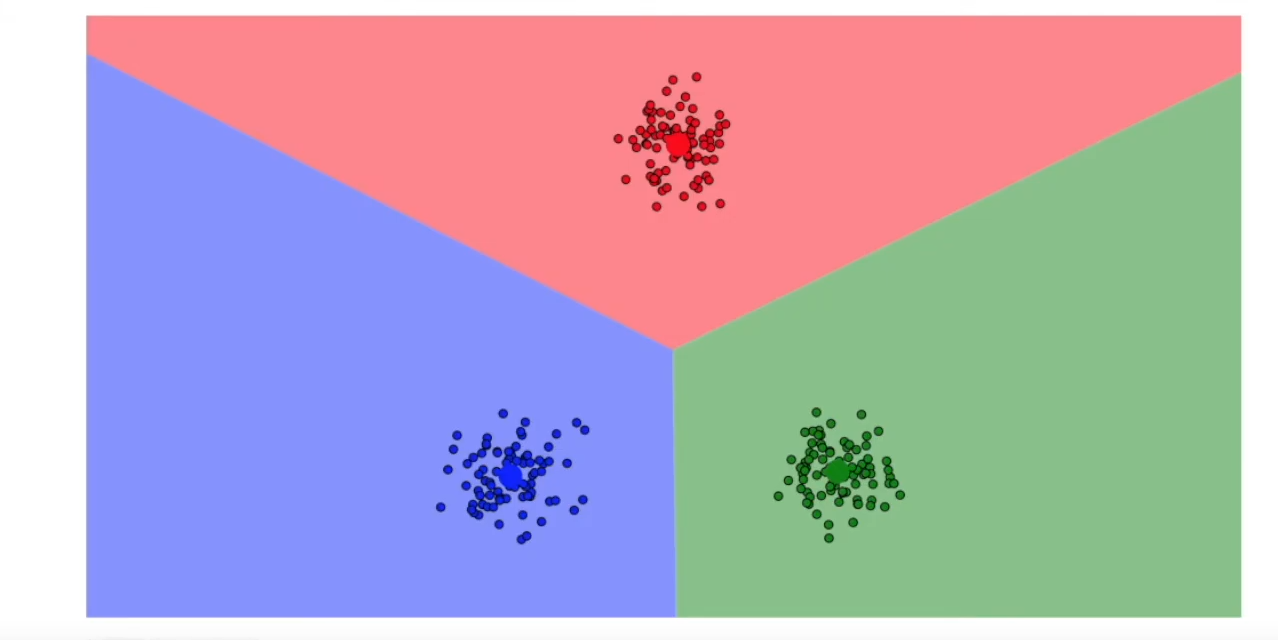
\includegraphics[width=0.99\textwidth,clip]{kmeans6.png}};
			\node (wiki)[visible on=<6>]  at([yshift = 13]ref.north) {Recalcul des centroïdes};
			%
			\node (ref) [visible on=<7>] {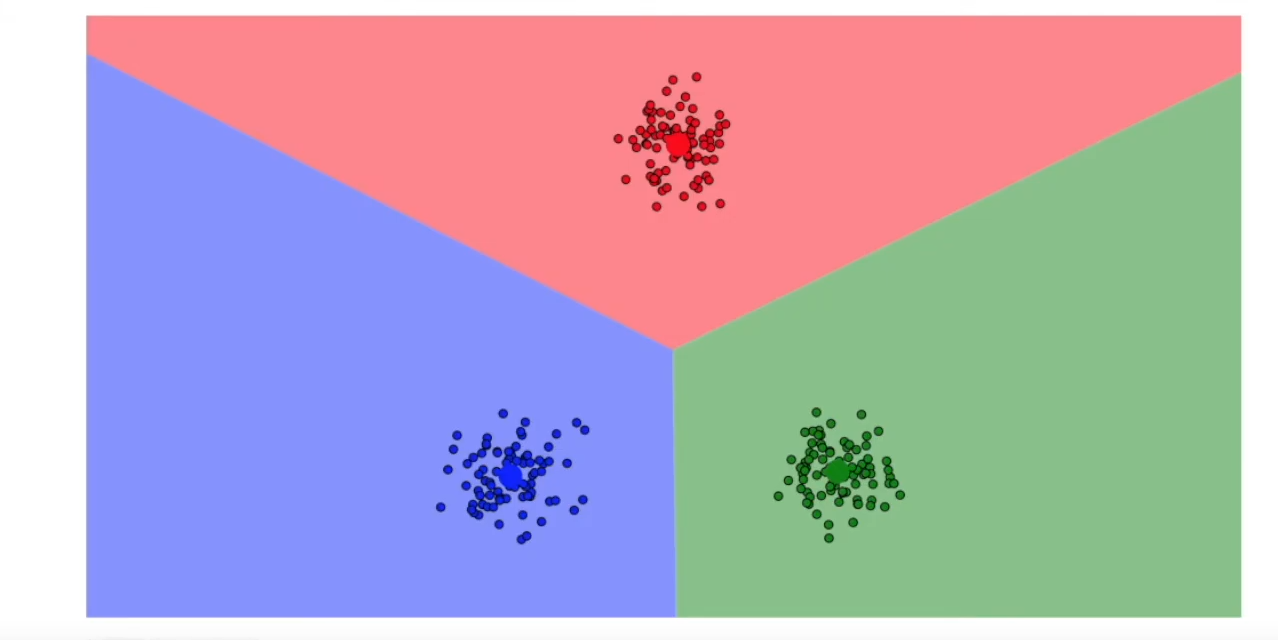
\includegraphics[width=0.99\textwidth,clip]{kmeans6.png}};
			\node (wiki)[visible on=<7>]  at([yshift = 13]ref.north) {Affectation des données au centroïde le plus proche : pas de changement};
			%
		\end{tikzpicture}
		
		%\vspace*{1.5em}
		\footnotesize{\textcolor{MPTgrey}{Tirée de la vidéo \textit{\href{https://www.youtube.com/watch?v=R2e3Ls9H_fc}{K-Means Clustering Explanation and Visualization}}} }
		
	\end{center}

\end{frame}
%------------------------------------------------------------------------------------------



%------------------------------------------------------------------------------------------
\begin{frame}{Répétition de la procédure}


		\textcolor{MPTred}{\large\textbf{Proposition}} \\ 
	\vspace*{-0.2em}		
	\begin{valblock}{}
		L’inertie intra-classes 
		$$\displaystyle\sum_{k=1}^K  \sum_{x \in \C_k} \|x-\mu_k\|^2$$
		diminue à chaque itération de l’algorithme
	\end{valblock}	
\footnotesize{\textcolor{MPTgrey}{voir preuve du lemme 22.1 de l'ouvrage \textit{\href{https://www.cs.huji.ac.il/~shais/UnderstandingMachineLearning/understanding-machine-learning-theory-algorithms.pdf}{Understanding Machine Learning: From Theory to Algorithms}}} }
\normalsize
	\vspace*{1em}
\begin{minipc}[0.1]{0.15}
	\warning
\end{minipc}
\begin{minipc}[0.89]{0.15}
	Il est donc possible de tomber dans un minimum local 
\end{minipc}
\begin{minipc}[0.1]{0.15}
	%\begin{center}
	\raisebox{1.5mm}{\bclampe \xspace} 
\end{minipc}
\begin{minipc}[0.89]{0.15}
	Afin d'améliorer les performances de l'algorithme des $K$-moyennes, il est souvent recommandé de répéter la procédure plusieurs fois avec différentes initialisations aléatoires des centroïdes
\end{minipc}
	
\end{frame}
%------------------------------------------------------------------------------------------
%------------------------------------------------------------------------------------------
\begin{frame}{Choix de $\color{MPTblue} K$}
	\vspace*{-0.5em}
				Le nombre de cluster $K$ est un hyperparamètre de l'algorithme des $K$-moyennes à choisir. Ce choix peut-être fait en minimisant un critère, comme l'inertie intra-classe\\[1em]					
	\begin{minipc}[0.06]{0.12}
		\warning 
		\end{minipc}
	\begin{minipc}[0.93]{0.12}
		l'inertie intra-classe va forcément diminuer plus $K$ augmente, pour autant, on ne veut pas choisir la partition avec $n$ clusters
	\end{minipc}
%
		\begin{minipc}[0.06]{0.2}
			%\begin{center}
			\raisebox{1.5mm}{\bclampe \xspace} 
		\end{minipc}
		\begin{minipc}[0.93]{0.2}
			Pour $K$ petit, on observe une décroissante forte de l’inertie intra-classes puis cette décroissante s’atténue au niveau d'un coude, là où l’on observe un changement de pente. On peut donc choisir $K$ au niveau du coude ; c'est le \textit{critère du coude}			
		\end{minipc}
		
	
	\begin{center}	
	
	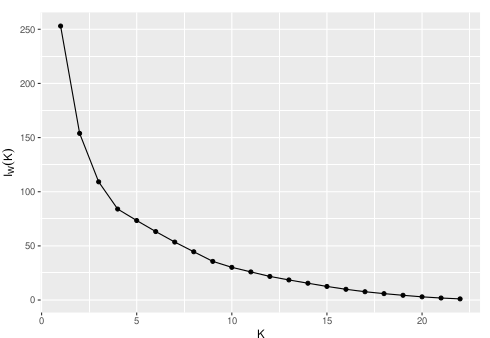
\includegraphics[width=0.4\textwidth]{Images/coude.png}
	
%	\vspace*{0.5em}
	\footnotesize{\textcolor{MPTgrey}{Le coude se situe autour de $\color{MPTgrey} K=4$}}
\end{center}
	
	
	
\end{frame}



%------------------------------------------------------------------------------------------
%------------------------------------------------------------------------------------------
\begin{frame}{Complexité algorithmique}

	À chaque itération, on calcule $K n$ distances en $d$ dimensions. Pour $t$ itérations, la complexité algorithmique de l’algorithme de Lloyd est donc en $O(ndKt)$.\\[1.2em]
	
	Puisque $K$
	et $t$ sont négligeables devant $n$, cet algorithme est donc linéaire en le nombre d’observations, par opposition au clustering hiérarchique dont le coût est quadratique en n (si l'on stocke les distances entre les observations). C'est expliqué par le fait que le calcul des distances d’une observation $x_i$ aux $n-1$ autres points du jeu de données a été remplacé par un calcul de sa distance à $K$ centroïdes\\[1.2em]
	
	Il est possible de combiner $K$-moyennes et clustering hiérarchique : on fait un $K$-moyennes avec $K=\lambda n$, une fraction importante des données, et ensuite on fait un clustering hiérarchique ascendant sur le résultat de l'algorithme des $K$-moyennes\\[1em]
\end{frame}
%------------------------------------------------------------------------------------------
%------------------------------------------------------------------------------------------
\begin{frame}{Données abberrantes}
	

	L’algorithme des $K$-moyennes est sensible aux données aberrantes. Si une observation $x_i$ est très éloignée des autres observations, elle se retrouvera seule dans un cluster, tandis que le reste des données sera partitionné en $K - 1$ clusters.\\[1.2em]
	
	Cependant, cela permet d’utiliser l’algorithme des $K$-moyenne pour détecter les observations aberrantes : ce sont celles qui sont seules dans un cluster.\\[2em]
	
	Le partitionnement en $K$-médoïdes est une méthode de partitionnement plus robuste vis-à-vis des données aberrantes. Le médoïde d'une classe est défini comme le point de la classe dont la dissimilarité moyenne avec tous les autres points de la classe est minimale, c'est-à-dire qu'il s'agit de l'observation la plus centrale de la classe.\\[2em]
	
\end{frame}
%------------------------------------------------------------------------------------------
%------------------------------------------------------------------------------------------

\begin{frame}{Remarques}
	\vspace*{-1em}
	\bftitle{Forme des clusters} \\[0.3em]
Les centroïdes des clusters trouvés par l’algorithme des $K$-moyennes forment un diagramme de Voronoï. Les clusters sont donc convexes.  \\[1em]


\begin{center}
	
	\begin{tikzpicture}
		\node (ref) [] {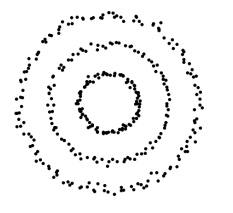
\includegraphics[width=0.3\textwidth,clip]{rond1.png}};
		\node (ref1) [right=of ref] {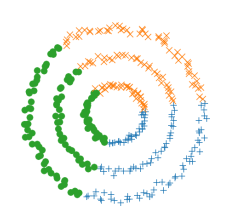
\includegraphics[width=0.3\textwidth,clip]{rond2.png}};
		%\node (wiki1)[]at([xshift = 30]wiki.east) {Non séparable linéairement};
		\node (wiki)[text width=4.3cm]  at([yshift = 7]ref1.north) {\small Partitionnement en 3 clusters
			par $K$-moyennes};
		
	\end{tikzpicture}
	
	%\vspace*{1.5em}
	\footnotesize{\textcolor{MPTgrey}{Tirée de l'ouvrage \textit{\href{http://cazencott.info/dotclear/public/lectures/IntroML_Azencott.pdf}{Introduction au Machine Learning}} de Chloé-Agathe Azencott} }\\[1.3em]
	
\end{center}

	\begin{minipc}[0.1]{0.1}
	%\begin{center}
	\raisebox{1.5mm}{\bclampe \xspace} 
\end{minipc}
\begin{minipc}[0.89]{0.1}
	On peut utiliser l'astuce du noyau à \textit{l’algorithme de Lloyd} pour obtenir des clusters non convexes \textcolor{MPTgrey} {(voir section 12.4.3 d'\textit{\href{http://cazencott.info/dotclear/public/lectures/IntroML_Azencott.pdf}{Introduction au Machine Learning}} de Chloé-Agathe Azencott)}
\end{minipc}
\end{frame}

%------------------------------------------------------------------------------------------
%------------------------------------------------------------------------------------------
%\begin{frame}{Méthode des $K$-moyennes avec noyau}
%	
%\end{frame}

\section{Évaluation d'un clustering}
%------------------------------------------------------------------------------------------
%------------------------------------------------------------------------------------------


\begin{frame}
	

	  Le clustering n’étant pas supervisé, il nous faut mettre au point des critères d’évaluation qui ne dépendent pas d’une vérité terrain (c’est-à-dire d’étiquettes connues). La tâche est plus délicate que dans
	le cadre de l’apprentissage supervisé, dans lequel le but à atteindre est beaucoup plus clair. Voici quelques manières de vérifier la qualité d'un clustering\\
	
	
	\vspace*{1em}
	\bftitle{Stabilités des clusters}\\[0.2em]
	On veut que le clustering soit robuste : collecter plus de
	données, perturber\\ ou supprimer quelques observations ou initialiser différemment l'algorithme de partitionnement ne devrait pas changer complètement les conclusions.\\[1em] 	
%	Ce dernier critère peut être utilisé pour choisir les hyperparamètres de l’algorithme : si on obtient des clusters très différents pour différentes initialisations de l’algorithme de partitionnement, cela peut indiquer que les hyperparamètres sont mal choisis.
	\bftitle{Évaluation externe}
	\begin{itemize}
		\item[\ex] \textbf{A posteriori}, un expert peut évaluer la qualité du clustering : les groupes sont-ils cohérents, ont-il du sens ?\\[0.2em]
		\item[\ex] \textbf{A priori}, si on dispose d'un jeu de données (partiellement) étiquetées, on peut vérifier si on retrouve les classes avec le clustering (\href{https://fr.wikipedia.org/wiki/Indice_de_Rand}{indice de Rand})
	\end{itemize}

	\vspace*{1em}
	\bftitle{Évaluation interne}
\begin{itemize}
	\item[\ex] On peut mesurer certaines statistiques comme l'indice de Davies-Bouldin global ou le coefficient de silhouette global enfin de se rendre compte de la qualité du partitionnement en terme d'homogénéité des clusters et de séparabilité entre les clusters
\end{itemize}
	
	
\end{frame}


%
%%------------------------NOTE
%\note{dire ici qu'on regarde quand $\X = \bbR^d$}
%
%	
%\end{frame}
%------------------------------------------------------------------------------------------
%------------------------------------------------------------------------------------------

\begin{frame}{Références}
	\begin{thebibliography}{2}
			\vspace{-1.8em}
			
	%	\bibitem{1} L.~Bel, J.N.~Bacro and C.~Lantuéjoul, \textcolor{black}{Assessing extremal dependence of environmental spatial fields,} \emph{Environmetrics}, 19(2):163-182, 2008
		
		\bibitem{pouet} C.A.~Azencot \textcolor{black}{{\href{http://cazencott.info/dotclear/public/lectures/IntroML_Azencott.pdf}{Introduction au Machine Learning}}}, \emph{Dunod},\\ ISBN : 978-2-10-084143-1\\[2em]
		
	%	\bibitem{CNP2006} D.~Cooley, P.~Naveau and P.~Poncet \textcolor{black}{Variograms for spatial max-stable random fields}, pages 370-390, \emph{Springer New-York}, 2006
		
		\bibitem{2} S.~Shalev-Shwartz and S.~Ben-David, \textcolor{black}{Understanding Machine Learning: From Theory to Algorithms,} \emph{Cambridge University Press}, DOI : 10.1017/CBO9781107298019, 2014\\[2em]
		%
	%	\bibitem{3} C.~Dombry, S.~Engelke, M.~Oesting (2016) \textcolor{black}{Exact simulation of max-stable processes}, \textit{Biometrika} 103(2):303–317
		
		\bibitem{E} T.~Hastie, R.~Tibshirani, and J.~Friedman. \textcolor{black}{The Elements of Statistical Learning}, \emph{Springer New York}, DOI : 10.1007/978-0-387-84858-7, 2009
		
		
		%
		%	\bibitem{4} R.A.~Fisher and L.H.C.~Tippett, \textcolor{black}{Limiting forms of the frequency distribution of the largest or smallest member of a sample,} \emph{Mathematical Proceedings of the Cambridge Philosophical Society}, 24(2):180-190, 1928\\[0.3em]
		%	
	\end{thebibliography}
	
\end{frame}
\end{document}
